\newpage
\visHeader

\subsection{Enterprise Architect Diagrams (Visual)}

\begin{itemize}
\FloatBarrier
\item[$\blacktriangleright$] Did\hypertarget{simpleDemo vis}{} you notice the new Demo.eap file in your package explorer? This is the EA file you'll be testing
and modelling your program with. Don't worry about the other folder and the exclamation mark it carries. The problems will be resolved by the end of this page.

In the meantime, Please do not rename, move, or delete anything.

\item[$\blacktriangleright$] Double click ``Demo.eap'' to start EA, and choose ``Ultimate" when starting EA for the first time.

\item[$\blacktriangleright$] In EA, choose ``Extensions/MOFLON::Ecore Addin/Export\- all\- to\- Workspace'' (Fig.~\ref{fig_ea}). Alternatively, you can activate
eMoflon's control panel window by selecting ``Extensions/Add-In Windows.'' Dock the dialog window that appears, and click ``Export/All'' within the `eMoflon
Global Functions' tab.

\vspace{1cm}

\begin{figure}[htbp]
	\centering
  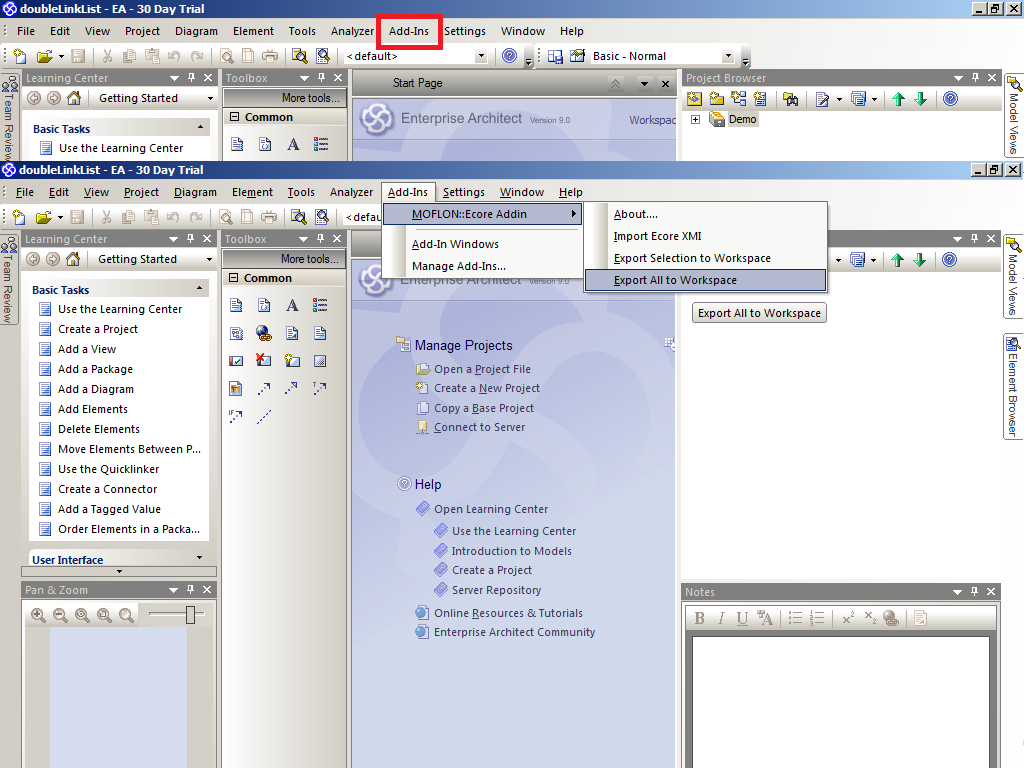
\includegraphics[width=0.9\textwidth]{ea_firststart}
	\caption{Export from EA using our extension} 
	\label{fig_ea} 
\end{figure}

\vspace{1cm}

\item[$\blacktriangleright$] Now try exploring the project browser! Try to navigate and understand some of the files and diagrams. This simple demo is meant to
familiarize you with visual representations classes, functions, and how they relate to eMoflon's generated code. Don't worry if you get confused - we provide
plenty of help and references throughout the handbook.
  
\item[$\blacktriangleright$] Switch back to Eclipse, choose your metamodel project, and press F5 to refresh. A new folder should appear, and your errors should
disappear after a few seconds. Since you've chosen to use our visual syntax, there isn't much to look at here. The export from EA places all required files in a
hidden folder(.temp) in the project, and refreshing triggers a build process that invokes our code generator automatically. You should be able to monitor the
progress with the green bar in the lower right corner. (Fig.~\ref{fig_eclipseBuild}) Pressing the symbol opens a monitor view that gives more details of the
build process. You don't need to worry about any of these details, just remember to refresh your Eclipse workspace after an export.

\item[$\blacktriangleright$] If you're ever worried about forgetting to refresh your workspace, or if you just don't want to bother with having to do this,
Eclipse does offer an option to do it for you automatically. To activate this, Go to ``Window/Preferences/General/Workspace" and select \texttt{refresh on
access}.

\fancyfoot[OR]{$\triangleright$ \hyperlink{validate common}{Next task}}

\vspace{2cm}

\begin{figure}[htbp]
	\centering
  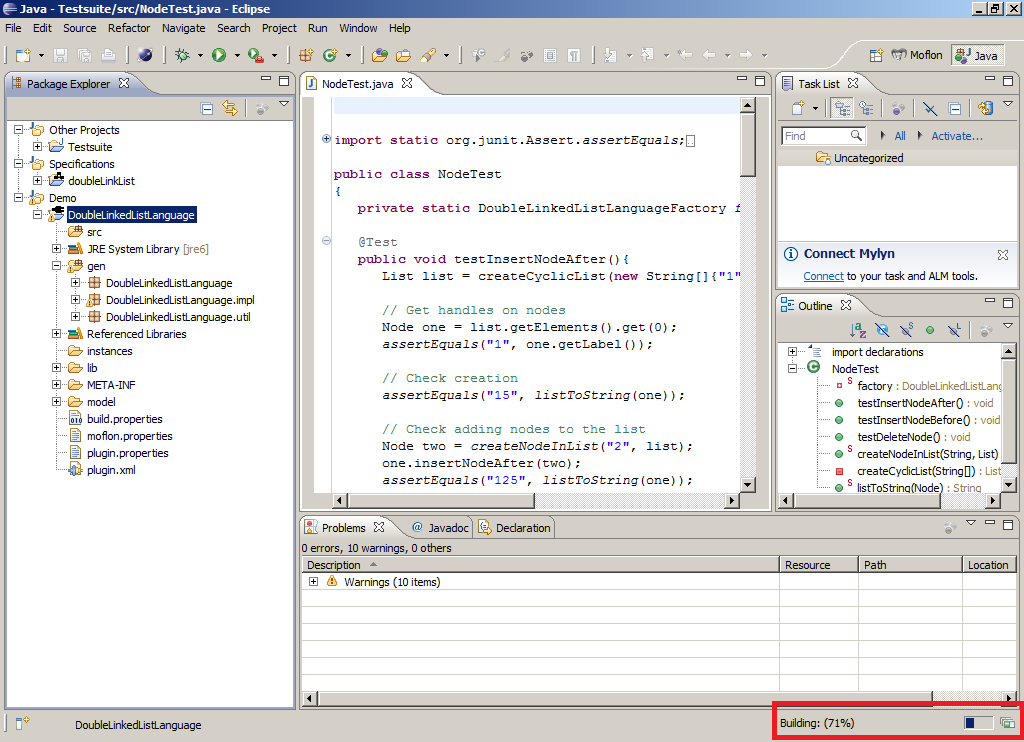
\includegraphics[width=0.9\textwidth]{eclipse_building}
	\caption{Eclipse: monitor project build} 
	\label{fig_eclipseBuild} 
\end{figure}

\end{itemize}